\begin{figure}[t]
    \centering

        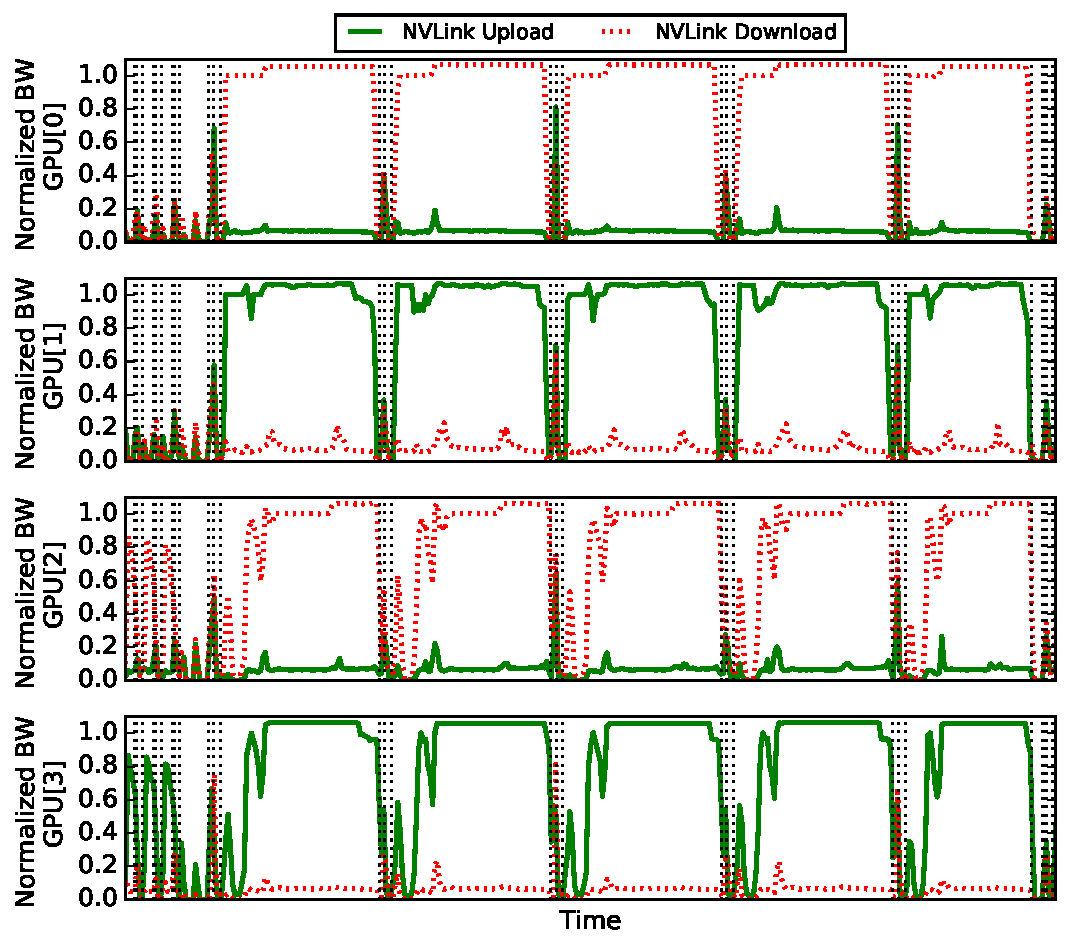
\includegraphics[width=1.0\columnwidth]{figures/bw_profile_HPGMG_UVM_base.pdf}
    \caption{Normalized NVLink bandwidth profile for HPC-HPGMG-UVM showing example of asymmetric 
    link utilization between GPUs and within a GPU depending on kernel and application phasing.}
    \label{fig:link-motivation}
\end{figure}

\section{Asymmetric Links for TMS-GPUS}
\label{interconnect}

Figure~\ref{fig:symmetric_assymetric}(a) shows a generic multi-socket system
with symmetric bandwidth assignments at each inter-socket communication link.
Static link capacity assignment at design time is very common and has multiple
advantages. For example, in such case only one type of I/O circuitry (egress
drivers or ingress receivers) along with only one type of control logic need to
be implemented at each on-chip interface. Moreover multi-socket switches a
result in simpler designs that support a statically provisioned worst-case
bandwidth scenario. On the other hand, multi-socket link bandwidth has a very
important impact on overall system perfromance as shown in
Figure~\ref{fig:switchtime}, where doubling NVLink capacity from 128GB/s to
256GB/s reached 1.5x average speedup reaching a 2x speedup for many
applications. As I/O bandwidth is a very limited and expensive resource, this
result motivates us to look for alternbatives that keep wire and I/O resources
at very high utilization. 



We note that the typically employed symmetric link
capacity asignments may result in lower overall utilization of the link wires
in many cases. Moreover, in case of TMS-GPU systems, we do observe that there
are applications in which some GPUs have a very different utilization of its
egress and ingress channels in different phases of execution.
Figure~\ref{fig:link-motivation} shows dynamic link utilization for a snapshot
of UVM version of HPGMG application running on our baseline 4 GPUs TMS-GPU
system. Vertical dotted black lines represent the beginning kernel calls that
are split across 4 GPUs as explained in Section~\ref{background}. We can see
that after few initial small kernels that have a negligible interconnect
utilization on all links, However for the the three larger kernels at the
figure GPU0 and GPU2 fully saturate their ingress links, while GPU1 and GPU3
fully saturate their egress links. At the same time GPU0 and GPU2 pair,
and GPU1 and GPU3 pair barely use their egress or ingress links accordingly.

\begin{figure}[t]
    \centering
    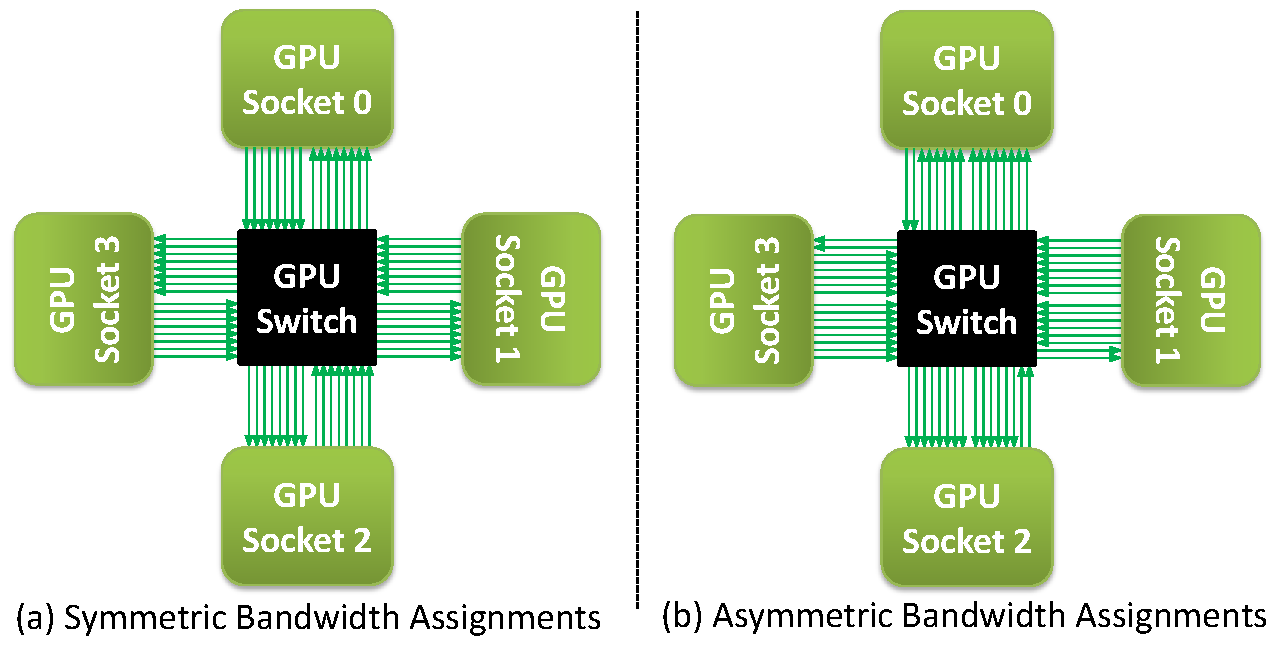
\includegraphics[width=1.0\columnwidth]{figures/tms_links.pdf}
    \caption{PLACEHOLDER FOR REAL FIG: Multi-socket systems with symmetric and
    assymeteric capacity assignments}
    \label{fig:symmetric_assymetric}
\end{figure}



Motivated by these findings, we propose to dynamically control multi-socket
link bandwidth assignments in each direction on a per-GPU basis resulting in
dynamically assymetric link capacity assignments as shown in
Figure~\ref{fig:symmetric_assymetric}(b). Such dynamic and assymetric link
capacity assignment is expected to yield higher wire utilization and
essentially higher effective bandwidth and perfromance for a given set of I/O
resources. This mechanism is somewhat similar to DRAM interface for example,
where the same set of wires is used for both read and write directions
interchangeably, and link direction is reversed based on a dynamic state of the
system. 

Specifically, for basic link configuration we assume and model point-to-point
links with multiple lanes each, similarly to NVLink
sub-links~\cite{pascal-tesla-wp}.  In such link, 8 lanes with 8GB/s capacity
per lane results in an aggregate bandwidth of 64GB/s in each direction. We
propose an adaptive assymetric scheme that works as following. For each link
in the system, at kernel launch we start with symmetric link assignments with 8
lanes per direction. Then, we propose to periodically sample the saturation
status of each link. If the lanes in one direction are not saturated, while the
lanes in the opposite direction are 99\% saturated, we reverse the direction of
one of the unsaturated lanes. We periodically repeat and sample the lanes
status, we stop either when equilibrium is reached, or alternatively all the lanes but one
have been reversed (we always keep a minimum bandwith of 8GB/s in each
direction).  
%We have a threshold of 
%1GB/sec to prevent switching for minimum variations in traffic shape.  
% EVGENY - I dint get it\ldots if you belive its importnat rephrase.  
There are two important factors that characterize the
behaviour above (i) \emph{switch\_time}: the cost of switching the direction a
lane (ii) \emph{sample\_time}: the frequency at which we want to sample for a
possible reconfiguration. The cost of switching a lane is comprised of the time
it takes to drain all the pending packets in a given diretion, and teh time it
takes to physically reconfigure the lane to start transmitting in the opposite
direction.

------  Evgeny : still need to add what are teh disadvnatages of assymetric
(double IO interfaces and switching complexity)

\begin{figure*}[tp]
    \centering
    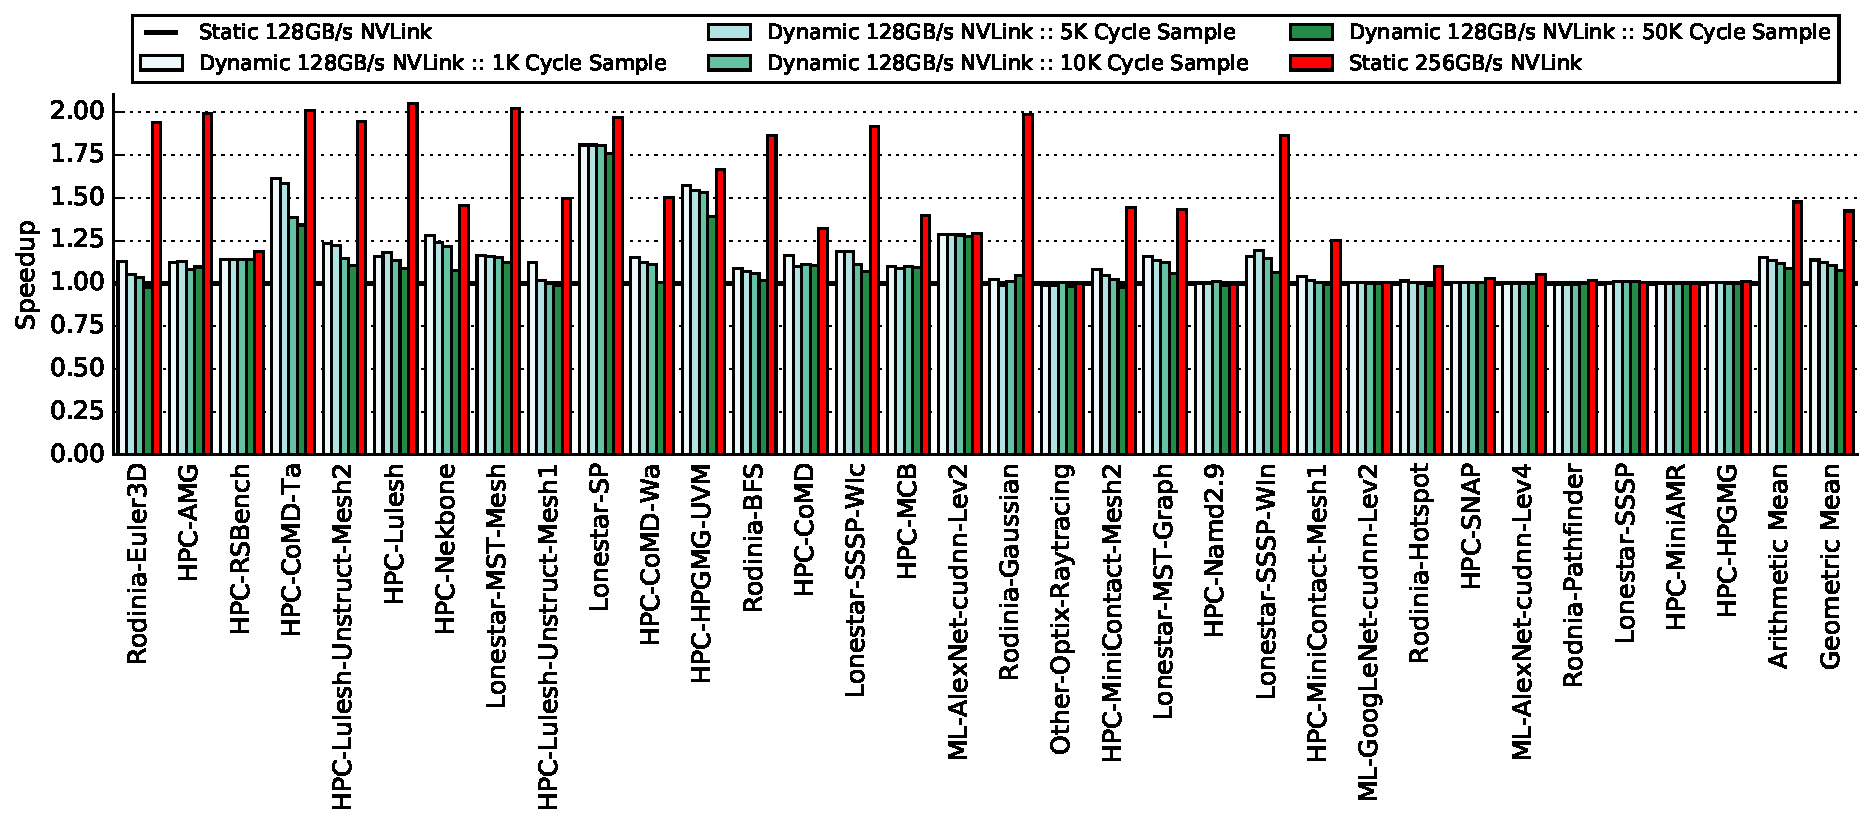
\includegraphics[width=1.0\textwidth]{figures/plot_nvlink_sample_time.pdf}
    \caption{Relative speedup of the dynamic NVlink adaptivity with respect to
	the baseline architecture by varying sample time and assuming switch time of
	100 cycles. In red, relative speedup achievable by doubling the bandwidth.}
    \label{fig:sampletime}
\end{figure*}


 \subsection{Results}
Figure~\ref{fig:sampletime} shows the expected performance improvement, with 
respect to our baseline architecture by exploring different values 
of the ``sample\_time'' and assuming a ``switch\_time'' of 100 cycles 
as reported in \cite{REALLY_NEED_REF_HERE}. Also in Figure~\ref{fig:sampletime}
we show with an upper-bound performance when doubling
the available interconnect bandwidth to 256GB/s (128GB/s per direction). 
We can see that for some applications the dynamic lane switching achieves up to
80\% improvements (``Lonestar-SP''). On average, even double the interconnect 
bandwidth we expect to see 50\% improvements while our dynamic solution 
achieves 15\% improvements. We can also see that the sample time plays a 
critical role and a too large sample time doesn't capture application dynamics 
resulting in smaller improvements. We found 5K cycles to be a reasonable sample
time able to achieve good results and never degrade performance. 
In Figure~\ref{fig:switchtime} we used 5K cycles sample time to
explore values of ``switch\_time'' from 10 cycles to 500 cycles.
We found that a faster switch does not produce better results than 100 cycles
but that in few applications a long (500 cycles) switch time results 25\% 
less performance with respect to 100 cycles (``HPC-CoMD-Ta'' and 
``HPC-CoMD-Wa'').

%when editing resuls, make sure we include more detail about variance to the switch time
%because we've removed the plot on it




% DO NOT REMOVE, we can use this to compute POWER later
%from http://teams.nvidia.com/sites/Corporate/ntech/SiteAssets/downloads/2014/NTECH2014_SlideDecks%20(presented)/7.1_Osborn.pptx
%Power: 8 lanes (TX + RX) at 25GT/s ~= 1.5W
%Area: 8 Lane PHY (8 TX + 8 RX + PLL) ~= 3.3mm^2
%Physical Data: .5pJ/b transferred




%REMOVING THIS FIGURE BECAUSE SWITCH TIME DOESN'T PROVIDE MUCH, SHOULD BE PUT
%IN TXT INSTEAD
%  \begin{figure*}[tp]
%     \centering
%     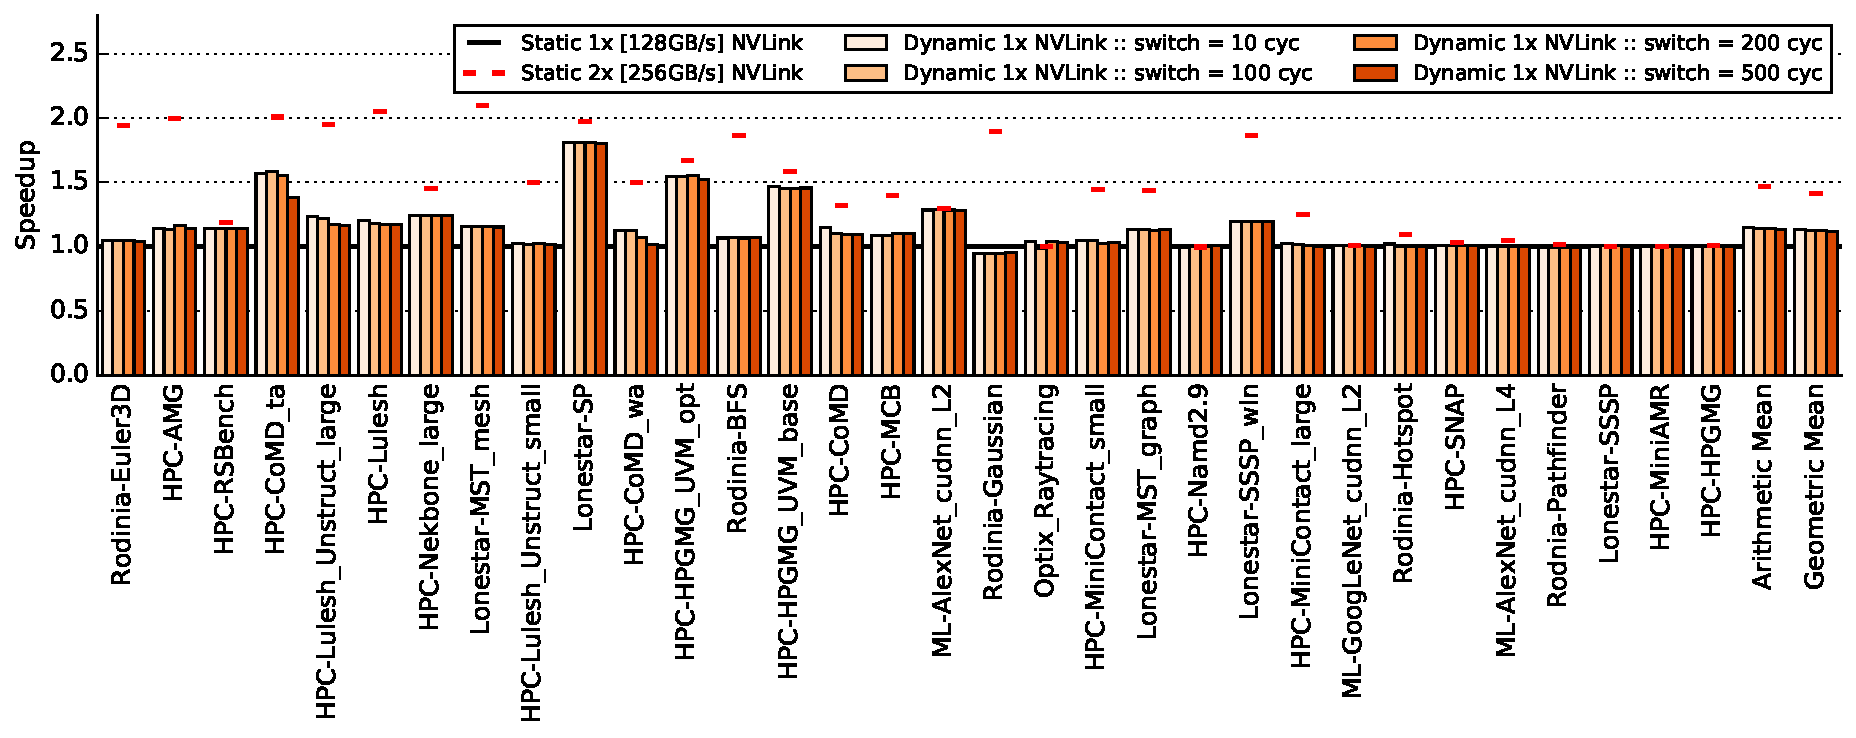
\includegraphics[width=1.0\textwidth]{figures/plot_nvlink_switch_time_sample_time5000.pdf}
%     \caption{Relative speedup of the dynamic NVlink adaptivity with respect to
% 	the baseline architecture varying switch time for a fixed sample time
% of 5k cycles. In red, relative speedup achievable by doubling the bandwidth.}
%     \label{fig:switchtime}
% \end{figure*}
